\documentclass[a4paper, 11pt]{article}
\usepackage{comment}
\usepackage{fullpage}
\usepackage{amsmath}
\usepackage{amssymb}
\usepackage{mathtools}
\usepackage{fontspec}
\defaultfontfeatures{Ligatures=TeX}
\usepackage{xfrac}
\usepackage{icomma}
\usepackage[section,below]{placeins}
\usepackage[labelfont=bf,font=small,width=0.9\textwidth]{caption}
\usepackage{subcaption}
\usepackage{graphicx}
\usepackage{grffile}
\usepackage{float}
\floatplacement{figure}{htbp}
\floatplacement{table}{htbp}
\usepackage{booktabs}
\usepackage{hyperref}
\usepackage[ngerman]{babel}
\usepackage{pdfpages}
\begin{document}
\noindent
%\centerline{\small{\textsc{Technische Universität Dortmund}}} \\
\large{\textbf{7. Übungsblatt zur Vorlesung \hfill WS 2017/2018 \\
Statistische Methoden der Datenanalyse \hfill Prof. W. Rhode}} \\
Annika Burkowitz, Sebastian Bange, Alexander Harnisch \\
\noindent\makebox[\linewidth]{\rule{\textwidth}{0.4pt}}


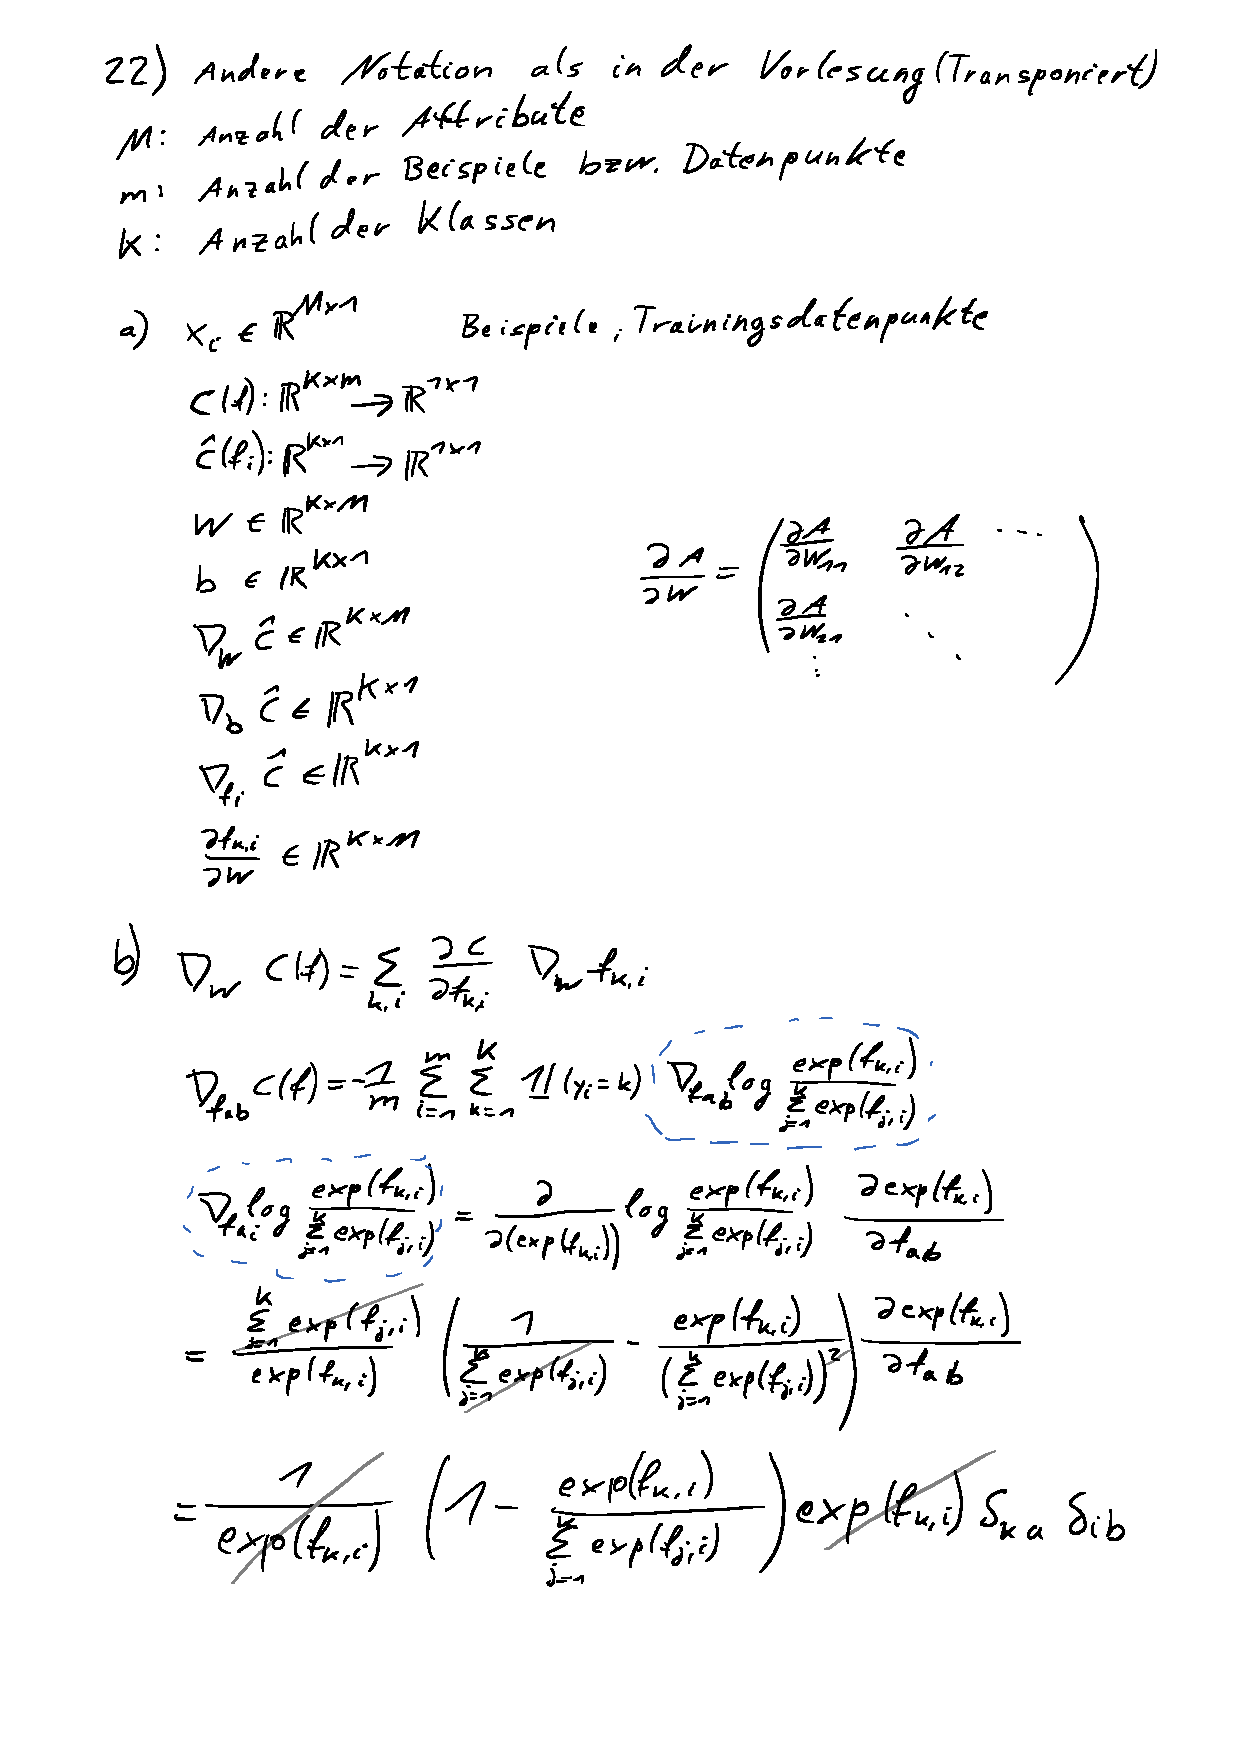
\includepdf[pages=1-3]{../Rechnungen.pdf}
\begin{figure}
    \centering
    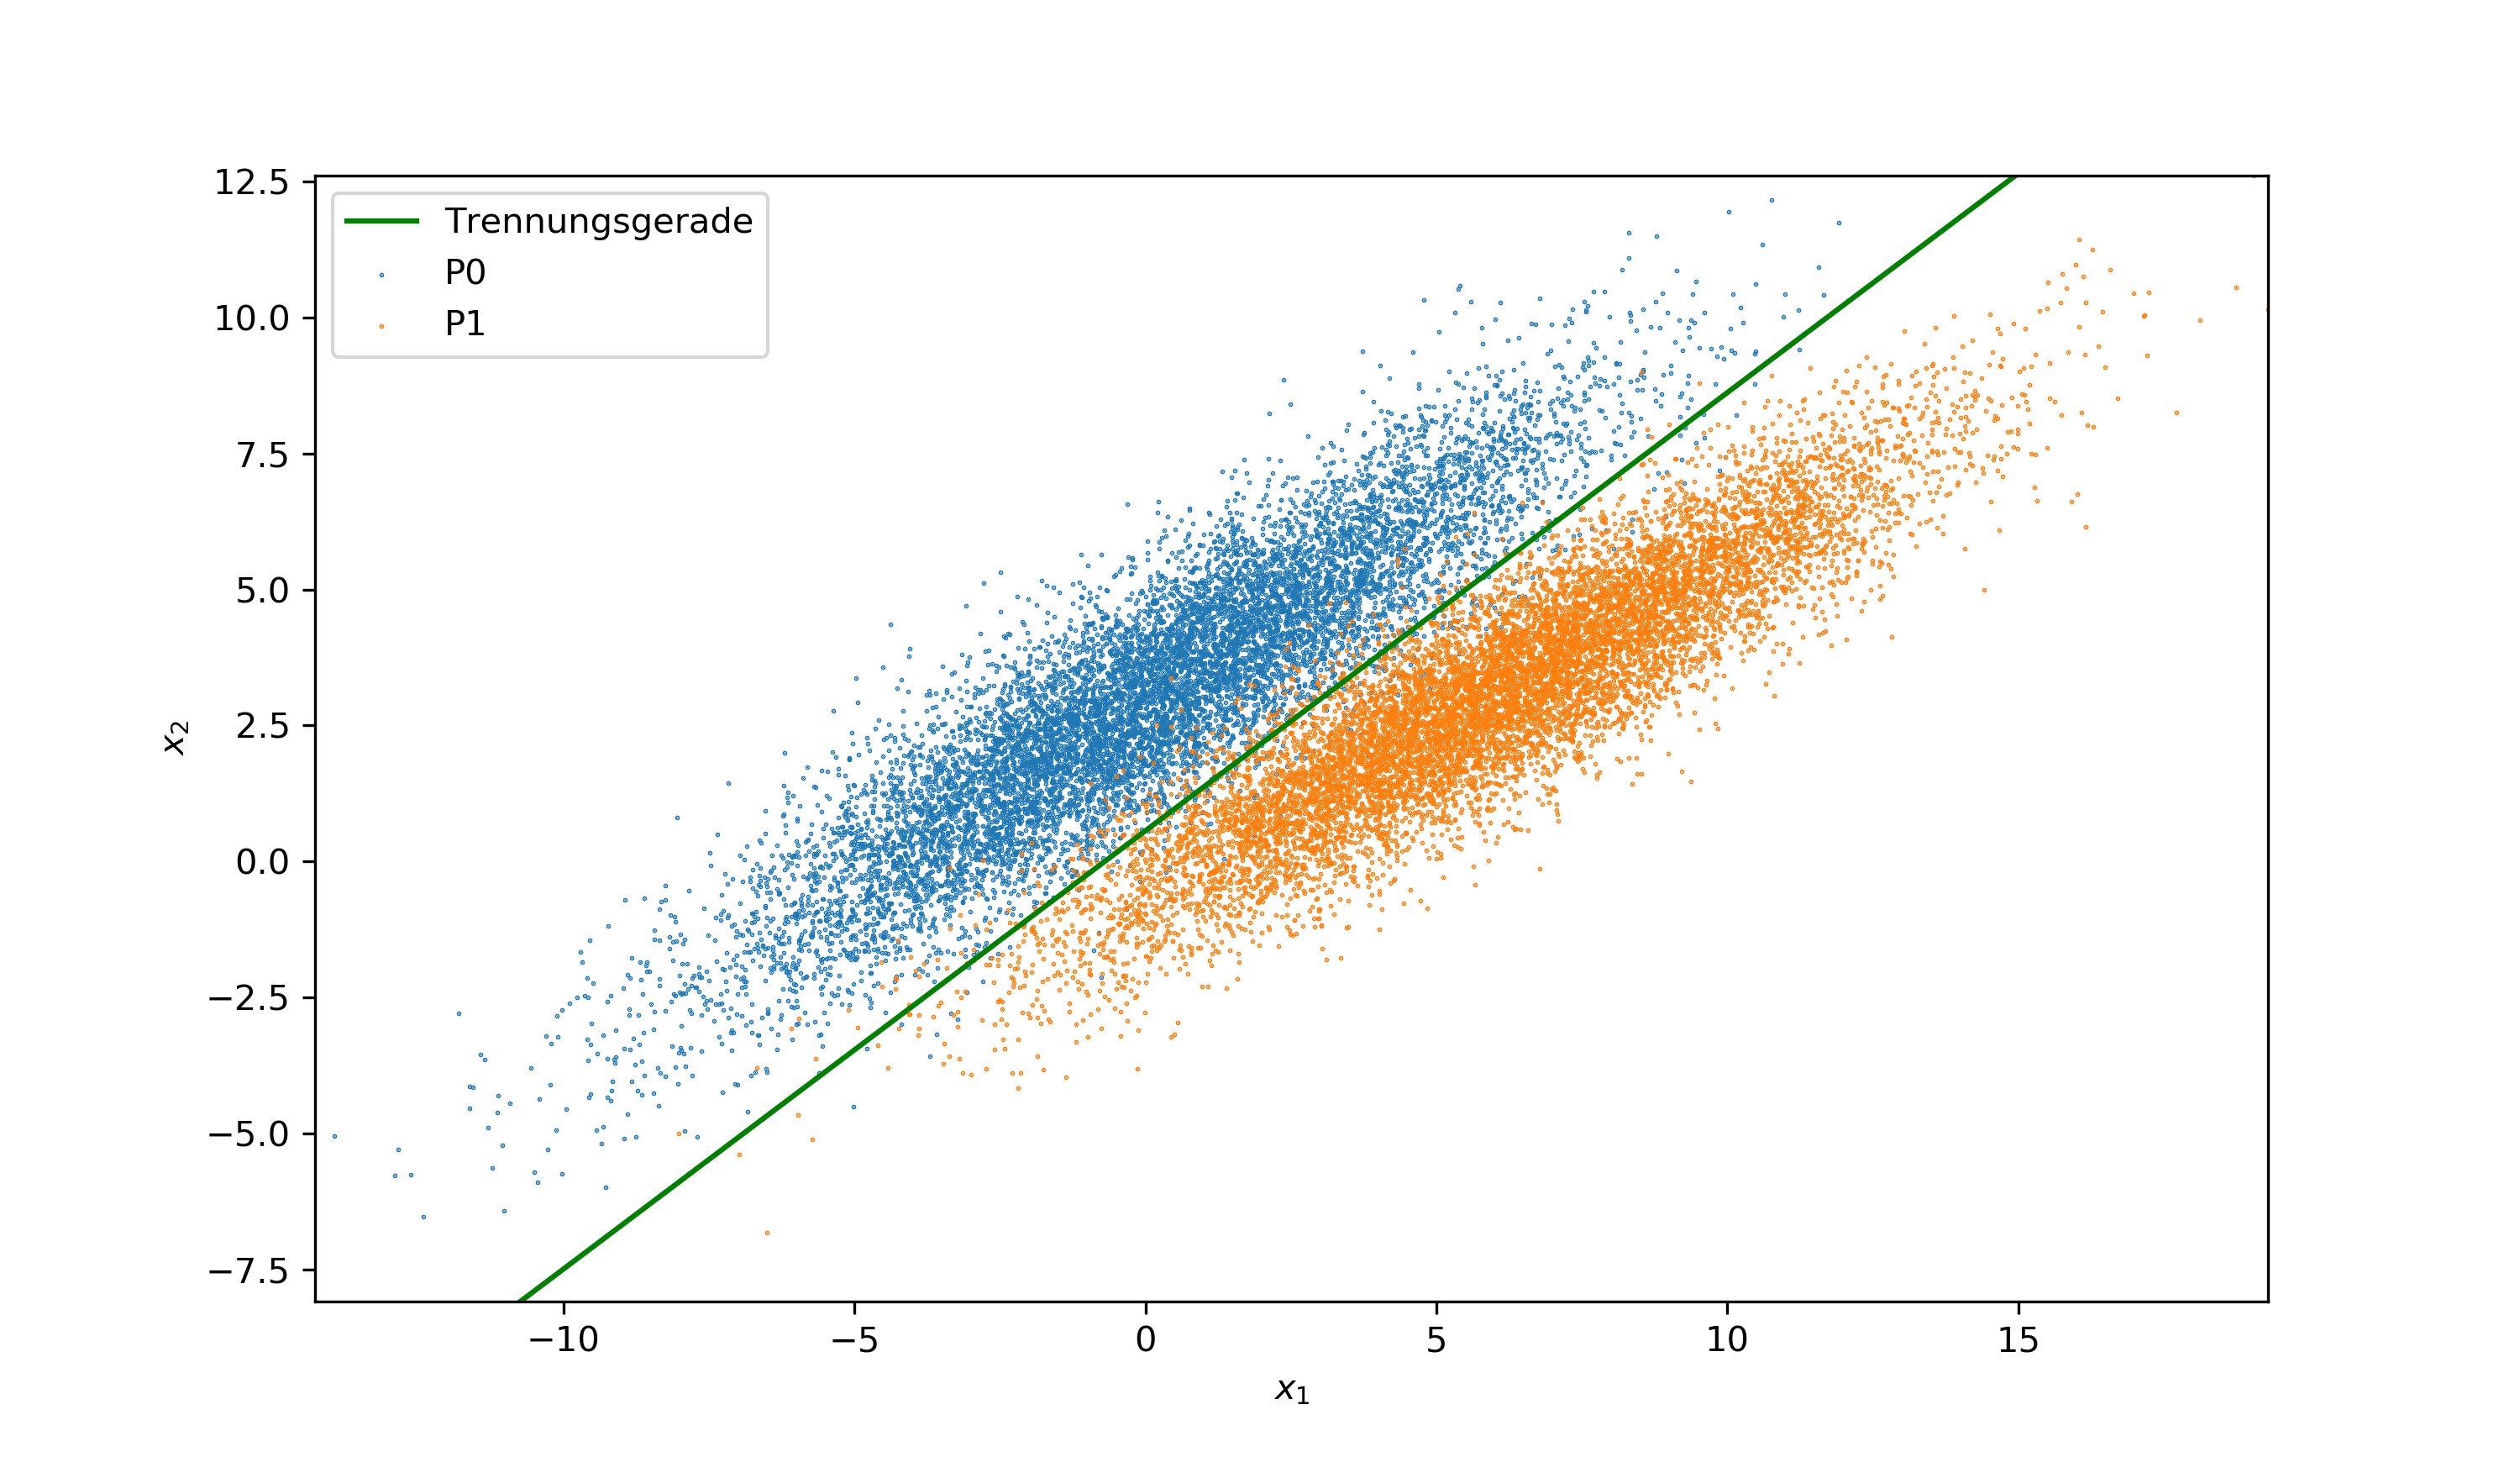
\includegraphics[width=\textwidth]{../A22/A22.png}
    \caption{Datenpunkte und Trenngrade.}
\end{figure}

\FloatBarrier
\includepdf[pages=4]{../Rechnungen.pdf}
\begin{figure}
    \centering
    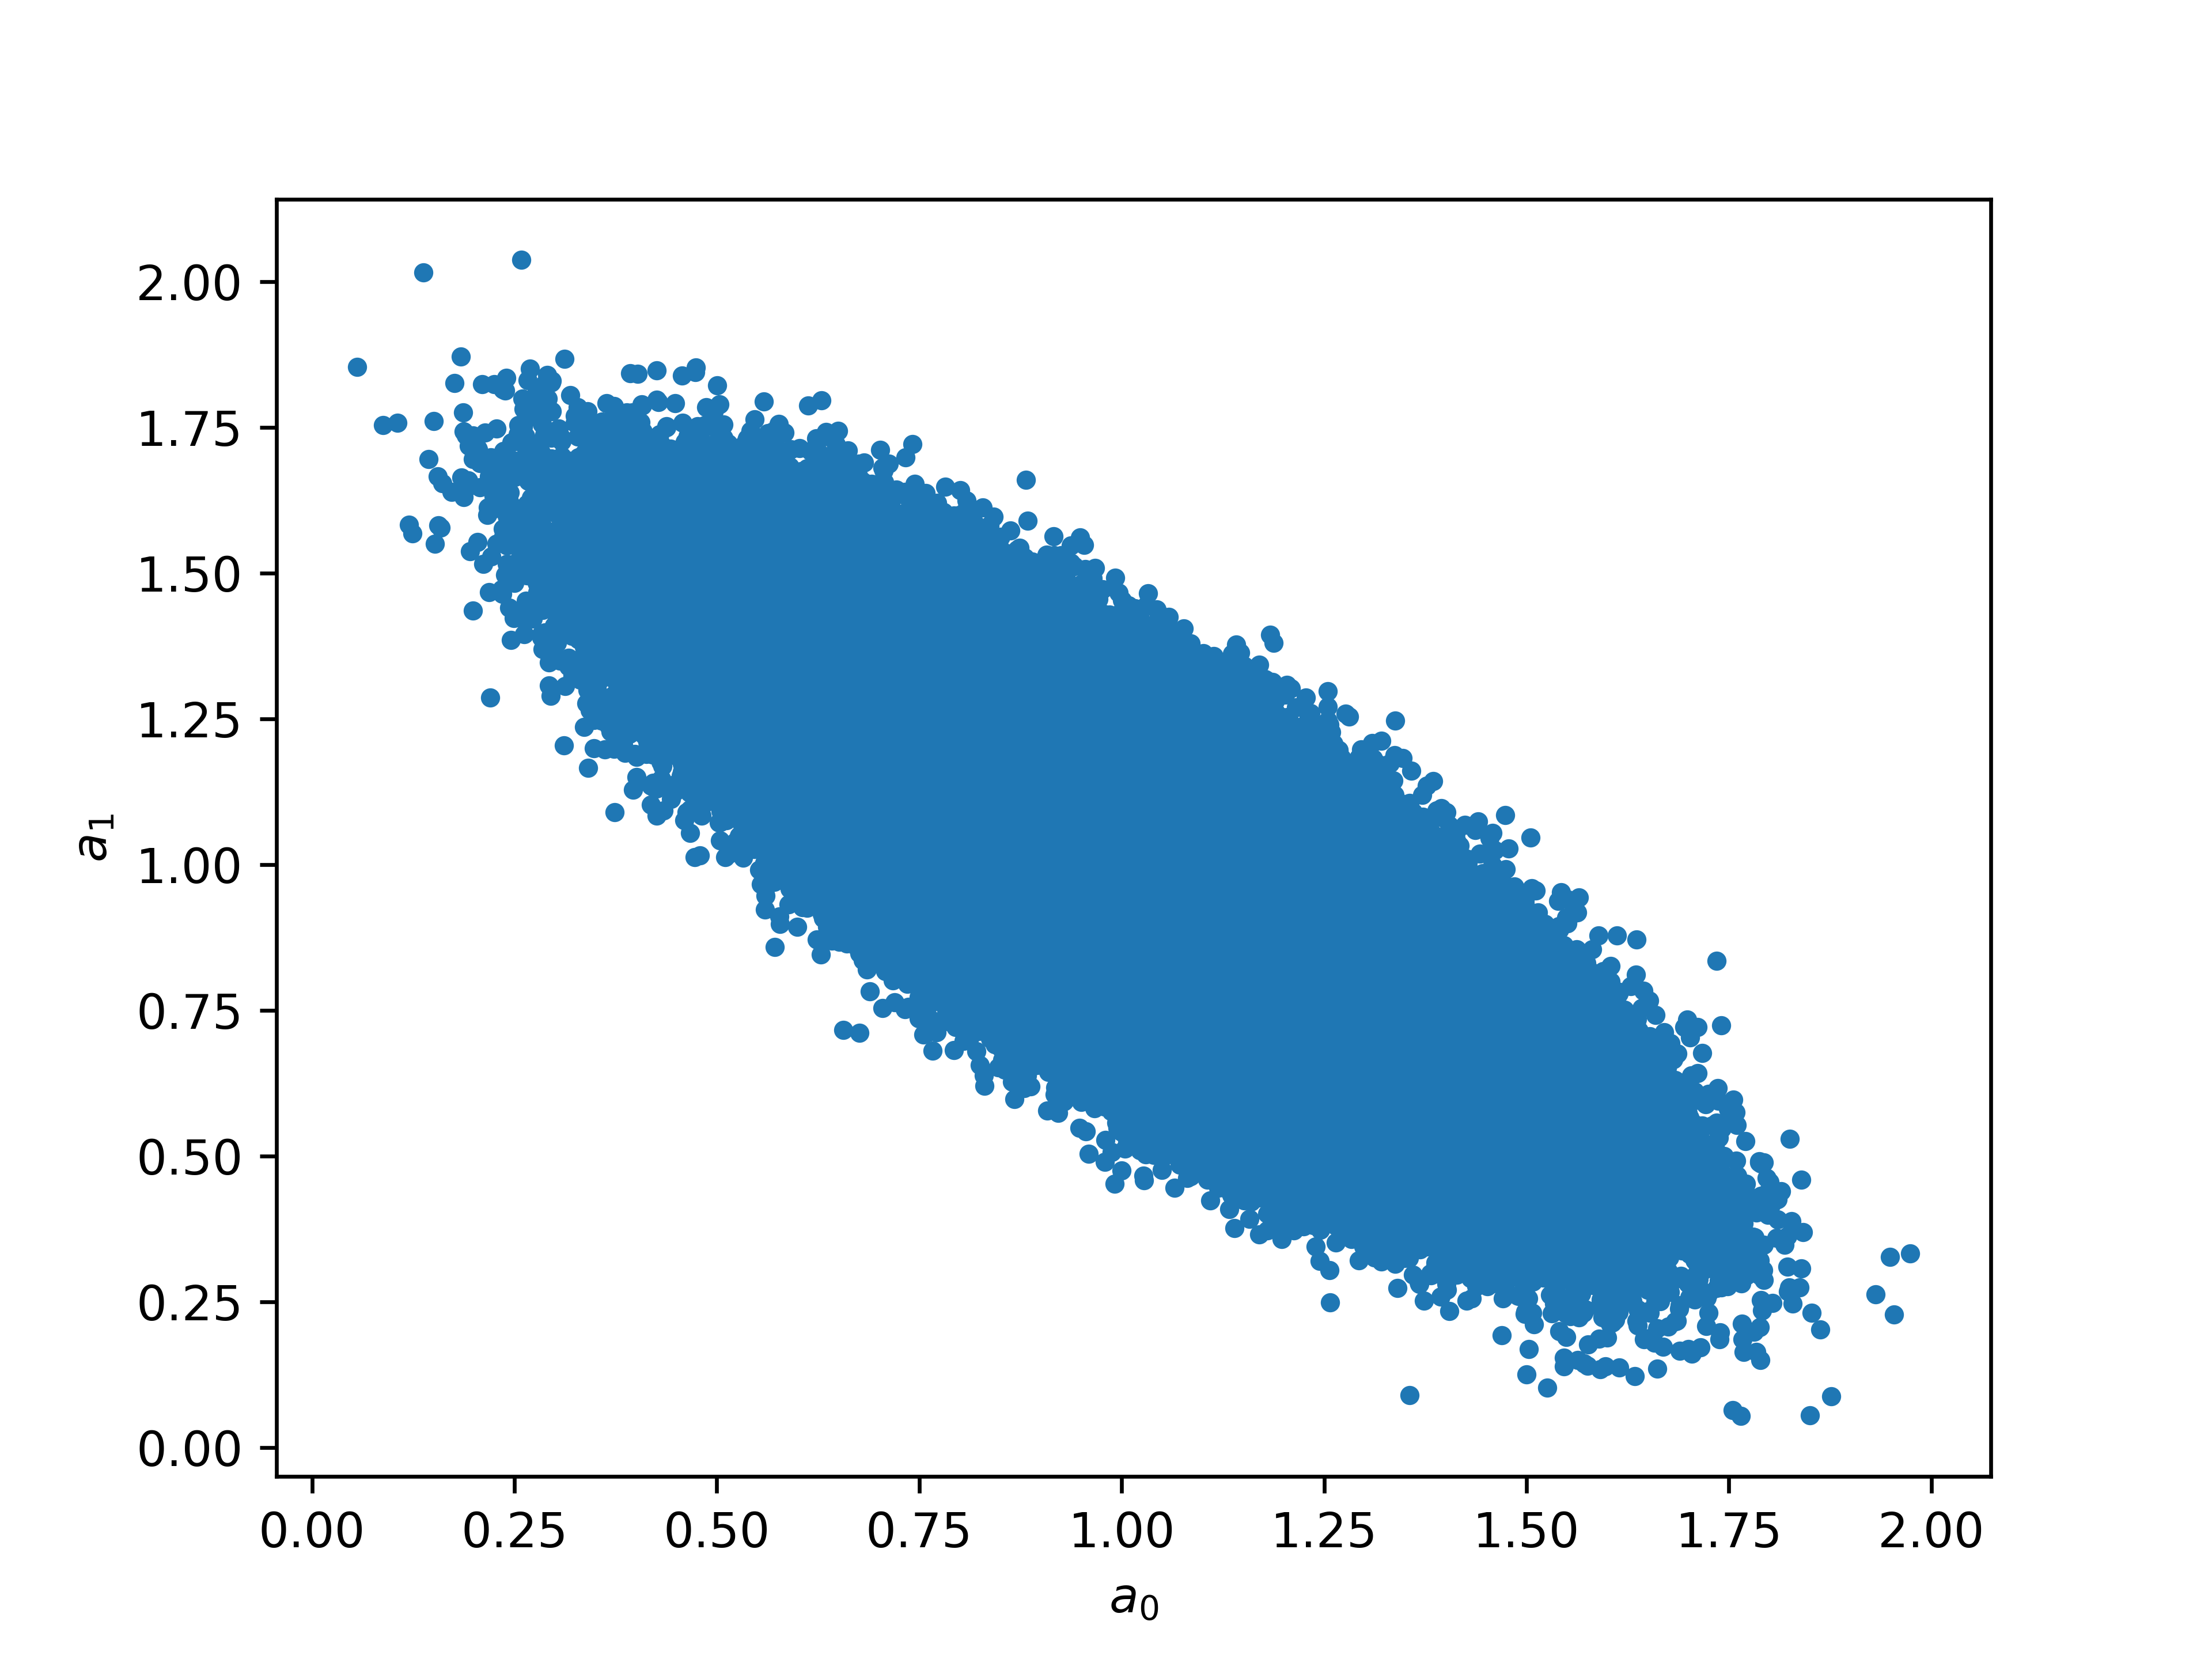
\includegraphics[width=\textwidth]{../A23/A23_scatter.png}
    \caption{Korrelierte Parameter $a_0$ und $a_1$.}
\end{figure}
\begin{figure}
    \centering
    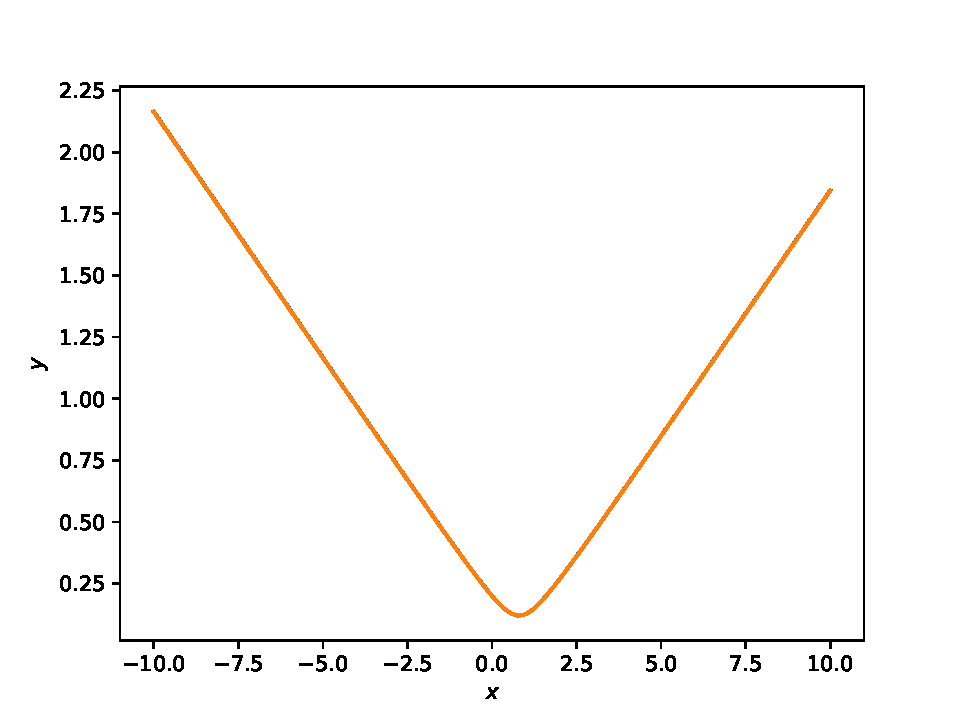
\includegraphics[width=\textwidth]{../A23/A23_resultat.pdf}
    \caption{Vergleich des numerisch bestimmten Fehlers mit dem analytisch bestimmten Fehlers.}
\end{figure}
\FloatBarrier

\section*{Aufgabe 24}
\subsection*{a)}
Die Lossfunktion gibt an, wie schlecht die berechnete Vorhersage im Vergleich
zu dem korrekten Ergebnis ist.
Um die bestmögliche Vorhersage zu treffen, muss die Lossfunktion minimiert werden.

\subsection*{b)}
Wenn die Lossfunktion abgeleitet werden kann, kann sie minimiert werden, in dem
die Ableitung der Lossfunktion gleich Null gesetzt wird.

\subsection*{c)}
Aktivierungsfunktionen stellen einen Zusammenhang zwischen dem Input an einem
Knoten in einem Neuronalen Netz und dem Output des Knotens her. Beispielsweise
realisieren sie einen Schwellwert für den Input, ab dem eine Aktivierung des
Neurons stattfindet und somit ein Output generiert wird.
Aktivierungsfunktionen sind nicht-linear und ermöglichen damit durch nicht-lineare
Kombination des (gewichteten) Inputs die Erzeugung nicht-linearer Entscheidungsgrenzen.
\newline
Beispiele
\begin{enumerate}
  \item Sigmoid:
   \begin{equation*}
     f(x)=\frac{1}{1+e^{-x}}
   \end{equation*}
  \item Tangens hyperbolicus:
   \begin{equation*}
     f(x)=\tanh(x)
   \end{equation*}
  \item Rectified Linear Unit (ReLU) / Softplus:
   \begin{align*}
     f(x)_\text{ReLU}&=\text{max}(0,x)\\
     f(x)_\text{Softplus}&=\ln\left(1+e^{x}\right)
   \end{align*}
  \item Softmax:
   \begin{equation*}
     q_k(x)=\frac{e^{f_k(x)}}{\sum_j e^{f_j(x)}}
   \end{equation*}
\end{enumerate}

\subsection*{d)}
Künstliche Neuronen sind Bestandteile eines Neuronalen Netzes. Jedes Neuron erhält
Input, der zunächst (mit individuellen Gewichtungen für jedes Neuron) gewichtet
wird und dann durch die Übertragungsfunktion aufsummiert wird. Das Ergebnis ist
die sogenannte Netzeingabe. Zusätzlich kann für jedes Neuron ein Schwellwert
festgelegt werden. Die Netzeingabe muss dann diesen Schwellwert überschreiten,
damit die Aktivierungsfunktion die Eingabe modulieren kann und somit die Ausgabe
festlegen kann.

\subsection*{e)}
Allgemein sind neuronale Netze dann besonders gut geeignet, wenn man selber die Lösung
nicht vernünftig mathematisch beschreiben kann.
Anwendungsbeispiele für Neuronale Netze:
\begin{enumerate}
  \item Bilderkennung: Wie definiert man einen Stuhl? Lösung: Das neuronale Netz soll sich
  das selber benennen.
  \item Spiele: Sehr viele mögliche Parameter, Problem wird zu hochdimensional.
  \item Sinnerkennung von Sprache (Siri, Cortana, Alexa,..): Ähnlich wie Bilderkennung zur Erkennung der Worte und viele mögliche Parameter, weil jeder leicht anders formuliert.
\end{enumerate}

\end{document}
